% !TEX root = Thesis.tex
\section{Relational Model}
	In its most basic form, the relational data model is built upon sets and tuples.  Each of these sets consist of a set of finite possible values.  Tuples are constructed from these sets to form relations.
	
	\begin{defn}[Named Tuple]
	\label{def:named-tuple}
		A named tuple $t$ is an instance of a relation $\gls{r}$, consisting of values corresponding to the attributes of $\gls{r}$.  For example,
		
		$$t = \left\{\mathrm{name}: \textrm{``Superman''}, \mathrm{age}: 33, \mathrm{birthplace}: \textrm{``Krypton''}\right\}$$
		
		We denote the attributes of $t$ as $\fcn{ATTR}{t} = \left\{\mathrm{name}, \mathrm{age}\right\}$  The values are $t\lbrack \mathrm{name}\rbrack = \textrm{``Superman''}$, $t\lbrack \mathrm{age}\rbrack = 33$, and $t\lbrack \mathrm{birthplace}\rbrack = \textrm{``Krypton''}$,
	\end{defn}
	
	\begin{defn}[Relation]
	\label{def:relation}
		A relation $r$ is a set of named tuples, $r = \left\{t_1, t_2, \dotsc, t_n\right\}$, such that all the named tuples share the same attributes.
		
		$$\forall t, t' \in r, \fcn{ATTR}{t} = \fcn{ATTR}{t'}$$
		
		For example,
		
		$$r = \left\{
			\begin{array}{l}
				\left\{\mathrm{name}: \textrm{``Superman''}, \mathrm{age}: 33, \mathrm{birthplace}: \textrm{``Krypton''}\right\}, \\
				\left\{\mathrm{name}: \textrm{``Batman''}, \mathrm{age}: 30, \mathrm{birthplace}: \textrm{``Earth''}\right\}, \\
				\left\{\mathrm{name}: \textrm{``Flash''}, \mathrm{age}: 53, \mathrm{birthplace}: \textrm{``Earth''}\right\}, \\
				\left\{\mathrm{name}: \textrm{``Wonder Woman''}, \mathrm{age}: 28, \mathrm{birthplace}: \textrm{``Earth''}\right\}, \\
				\left\{\mathrm{name}: \textrm{``General Zod''}, \mathrm{age}: 42, \mathrm{birthplace}: \textrm{``Krypton''}\right\}
			\end{array}
		\right\}$$
		
		Relations are typically represented as tables.
		
		\begin{table}[!ht]
			\centering
			\begin{tabular}{lll}
				\toprule
				name & age & birthplace \\
				\midrule
				Superman & 33 & Krypton \\
				Batman & 30 & Earth \\
				Flash & 53 & Earth \\
				Wonder Woman & 28 & Earth \\
				General Zod & 42 & Krypton \\
				\bottomrule
			\end{tabular}
			
			\caption{Person table}
			\label{tbl:person}
		\end{table}
	\end{defn}
	
	\begin{defn}[Keys]
	\label{def:keys}
		Keys are constraints imposed on relations.  A key constraint $K$ on a relation $r$ is a subset of $\fcn{ATTR}{r}$ which may uniquely identify a tuple.  Formally, we say $r$ satisfies the key constraint $K$, denoted as $r \models K$, subject to
		
		$$\forall t, t' \in r, t \not= t' \implies t[K] \not= t'[K]$$
		
		For example, in Table~\ref{tbl:person}, the relation satisfies the key constraint $\left\{\mathrm{name}\right\}$, but not $\left\{\mathrm{age}\right\}$.
	\end{defn}
	
	\begin{defn}[Foreign Keys]
	\label{def:foreign-keys}
		A foreign key constraint applies to two relations, $r_1, r_2$.  It asserts that values of certain attributes of $r_1$ must appear as values of some corresponding attributes of $r_2$.  A foreign key constraint is written as
		
		$$\theta = r_1(a_1, a_2, \dotsc, a_k) \rightarrow r_2(b_1, b_2, \dotsc, b_k)$$
		
		where $a_i \subseteq \fcn{ATTR}{r_1}$ and $b_i \subseteq \fcn{ATTR}{r_2}$.  We say $(r_1, r_2)$ satisfies $\theta$, denoted as $(r_1, r_2) \models \theta$, if
		
		$$\forall t \in r_1, \exists t' \in r_2 \mid t\lbrack a_1, a_2, \dotsc, a_k\rbrack = t'\lbrack b_1, b_2, \dotsc, b_k]$$
		
		\begin{ex}
			Suppose we have a relation Superhero(name, superpower).  We can impose a FK constraint of
			
			$$\textrm{Superhero(name)} \rightarrow \textrm{Person(name)}$$
		\end{ex}
	\end{defn}
	
	\begin{defn}[Relational Database]
	\label{def:relational-database}
		A relational database, $d$, is a named collection of relations (as defined by Definition~\ref{def:relation}, keys (as defined by Definition~\ref{def:keys}), and foreign key constraints (as defined by Definition~\ref{def:foreign-keys}.
		
		We use $\fcn{Name}{d}$ to denote the name of $d$, $\fcn{Rel}{d}$ the list of relations in $d$, $\fcn{Key}{d}$ the list of key constraints of $d$, and $\fcn{FK}{d}$ the list of foreign key constraints of $d$.
	\end{defn}
	
	\subsection{Schema Group}
		\begin{defn}[Schema Graph]
			If we view relations as vertices, and foreign key constraints as edges, a database $d$ can be viewed as a \emph{schema graph} $G$, formally defined as
			
			\begin{eqnarray*}
				\mathrm{vertices}:  V(G) &=& \fcn{REL}{d} \\
				\mathrm{edges}:  E(G) &=& \fcn{FK}{d}
			\end{eqnarray*}
		\end{defn}
		
		\begin{ex}
			Given the following schema
			
			\begin{figure}[!ht]
				\centering
				
				Superhero(\underline{name}, power) \\
				Person(\underline{name}, age, birthplace) \\
				Planet(\underline{name}, size, age, destroyed, galaxy) \\
				Link(\underline{name}, peer, relation type) \\
			\end{figure}
			
			and the following foreign key constraints
			
			\begin{eqnarray*}
				\textrm{Superhero(name)} &\rightarrow& \textrm{Person(name)} \\
				\textrm{Person(birthplace)} &\rightarrow& \textrm{Planet(name)} \\
				\textrm{Link(name)} &\rightarrow& \textrm{Person(name)} \\
				\textrm{Link(peer)} &\rightarrow& \textrm{Person(name)}
			\end{eqnarray*}
			
			we produce the following schema graph
			
			\begin{figure}[!ht]
				\centering
				
				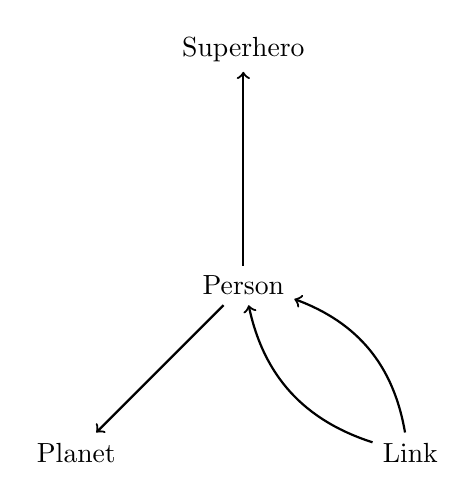
\begin{tikzpicture}[->,node distance=3cm,thick,main node/.style={rectangle,thick}]
					\node[main node] (Superhero)						{Superhero};
					\node[main node] (Person)	[below of=Superhero]	{Person};
					\node[main node] (Planet)	[below left of=Person]	{Planet};
					\node[main node] (Link)		[below right of=Person]	{Link};
					
					\path
						(Person)	edge node [right]					{}	(Superhero)
									edge node [left]					{}	(Planet)
						(Link)		edge [bend left]	node [left]		{}	(Person)
									edge [bend right]	node [right]	{}	(Person);
				\end{tikzpicture}
			\end{figure}
		\end{ex}
		
		The relational data model is particularly powerful for analytic queries.  Given the schema below above, one can formulate the following analytic queries in a query language known as SQL.
			
		\begin{ex}
			List all superheroes whose home planet has not been destroyed.
			
			\begin{figure}[!ht]
				\begin{singlespaced}
					\begin{sqlcode}
SELECT Person.name
FROM   Person
       JOIN Planet
         ON Person.birthplace = Planet.name
WHERE  NOT Planet.destroyed;
					\end{sqlcode}
				\end{singlespaced}
				
				\caption{Query to find superheroes with a home to go back to}
			\end{figure}
			
			Results in the following output, given the data from Table~\ref{tbl:person},
			
			\begin{table}[!ht]
				\centering
				
				\begin{tabular}{l}
					\toprule
					name \\
					\midrule
					Batman \\
					Flash \\
					Wonder Woman \\
					\bottomrule
				\end{tabular}
			\end{table}
		\end{ex}
		
	\subsection{Entity Group}
		\begin{defn}[Entity Group]
			An entity group is a forest, $T$,  of tuples interconnected by join conditions defined by the foreign key constraints in the schema graph.  Given two vertices $t_1, t_2'\in V\left(T\right)$, it must be that:

			$\exists r_1, r_2\in \fcn{REL}{d}$ such that $t_1 \in r_1$, $t_2\in r_2$, and $\left(r_1, r_2\right)\in G$.  This is to say that $t_1$ and $t_2$ belong to two relations that are connected by the schema graph.

			Let $r_1\left(a_1, \dotsc, a_k\right) \to r_2\left(b_1, \dotsc, b_k\right)$ be the FK that connects $r_1, r_2$.  We further assert that $t_1\lbrack a_1, \dotsc, a_k\rbrack = t_2\lbrack b_1, \dotsc, b_k\rbrack$.
		\end{defn}
		
		The motivation of entity groups is to define complex structured objects that can include more information than individual tuples in the relations.
		
		\begin{ex}
			The information in Table~\ref{tbl:superman-properties} all relates to Superman, however no single tuple in the database has all of this information as a result of database normalization.
			
			\begin{table}[!ht]
				\centering
				
				\begin{tabular}{ll}
					\toprule
					Attribute & Value \\
					\midrule
					name & Superman \\
					age & 33 \\
					birthplace & Krypton \\
					superpower & flying, strength, speed \\
					friends & Wonder Woman, Batman \\
					enemies & General Zod \\
					\bottomrule
				\end{tabular}
				
				\caption{Superman's properties}
				\label{tbl:superman-properties}
			\end{table}
			
			We require an entity group (Figure~\ref{fig:superhero-entity-group}) to join together all pieces of information related to Superman.
			
			\begin{figure}[!ht]
				\centering
				
				\begin{forest}
					[$\bowtie$
						[Link]
						[$\bowtie$
							[Superhero]
							[$\bowtie_{\mathrm{birthplace=Planet.name}}$
								[Planet]
								[$\sigma_{\mathrm{name=Superman}}(\mathrm{Person})$]
							]
						]
					]
				\end{forest}
				
				\caption{Superhero entity group}
				\label{fig:superhero-entity-group}
			\end{figure}

		\end{ex}

	\subsection{Pros and Cons of the Relational Model}
		In order to better understand the motivation behind this work, it is important to examine both the strong and weak points of the relational model.
		
		\subsubsection{Pros}
			The relational model was first proposed by Edgar F. Codd in 1969 while working at IBM \cite{codd-69}.
			
			The enforcement of constraints is essential to the relational model.  There are several types of constraints.  The first constraint maintains uniqueness.
			
			The Person relation has the attribute name as its primary key.  In order for other relations to reference a specific named tuple, the name attribute must be unique.
			
			\begin{ex}[Unique Constraint]
			\label{ex:unique-constraint}
				Attempt to insert another person named ``Superman.''
				
				\begin{singlespaced}
					\begin{sqlcode}
INSERT INTO Person
VALUES      ('Superman',
             35,
             'Earth'); 
					\end{sqlcode}
				\end{singlespaced}
				
				The \gls{rdbms} enforces the primary key constraint on the \texttt{name} attribute, rejecting the insertion.
				
				\begin{verbatim}
ERROR:  duplicate key value violates unique constraint "person_pkey"
DETAIL:  Key (name)=(Superman) already exists.
				\end{verbatim}
			\end{ex}
			
			With the uniqueness of named tuples guaranteed (as demonstrated in Example~\ref{ex:unique-constraint}), we must ensure that any named tuples that are referenced actually exist.  If they do not, the database must not permit the operation to continue.  Doing so would lead to dangling references.
			
			\begin{ex}[Referential Integrity]
				Attempt to insert the superhero ``Aquaman'' with the superpower ``telepathy.''
				
				\begin{singlespaced}
					\begin{sqlcode}
INSERT INTO Superhero
VALUES      ('Aquaman',
             'telepathy'); 
					\end{sqlcode}
				\end{singlespaced}
				
				Again we see the \gls{rdbms} protecting the integrity of the data.
				
				\begin{verbatim}
ERROR:  insert or update on table "superhero" violates foreign
key constraint "superhero_name_fkey"
DETAIL:  Key (name)=(Aquaman) is not present in table "person".
				\end{verbatim}
			\end{ex}
			
			In addition to enforcing consistency, the relational model is capable of providing higher-level views of the data through aggregation.
			
			\begin{ex}[Aggregation (Simple)]
				Find the number of friends Superman has.
				
				\begin{singlespaced}
					\begin{sqlcode}
SELECT COUNT(*)
FROM   Link
WHERE  name = 'Superman'
       AND relationtype = 'friend'; 
					\end{sqlcode}
				\end{singlespaced}
			\end{ex}
			
			\begin{ex}[Aggregation (Group By)]
				List the number of enemies of each Person.
				
				\begin{singlespaced}
					\begin{sqlcode}
SELECT name,
       Count(name)
FROM   Link
WHERE  relationtype = 'foe'
GROUP  BY name; 
					\end{sqlcode}
				\end{singlespaced}
				
				The above query produces the following output.
				
				\begin{table}[!ht]
					\centering
					
					\begin{tabular}{ll}
						\toprule
						name & count \\
						\midrule
						Superman & 1 \\
						General Zod & 1 \\
						\bottomrule
					\end{tabular}
				\end{table}
			\end{ex}
			
			Information stored within a properly designed database is normalized.  That is, no information is repeated.
			
			\begin{ex}[Normalization]
				For example, suppose the planet Krypton is discovered to have been in the ``Xeno'' Galaxy rather than the ``Andromeda'' Galaxy.  If this information were not normalized, each person whose birthplace was Krypton would need to be updated.  Since this information is normalized, the following query will suffice.
				
				\begin{singlespaced}
					\begin{sqlcode}
UPDATE planet
SET    galaxy = 'Xeno'
WHERE  name = 'Krypton';
					\end{sqlcode}
				\end{singlespaced}
			\end{ex}
			
			The above examples are some of the most important reasons for choosing the relation model over others.  Unfortunately the relational model is not without its downsides.
		
		\subsubsection{Cons}
			While the relational model excels at ensuring data consistency, aggregation, and reporting, it is not suitable for every task.  In order to issue queries, a user must be familiar with the schema.  This requires specific domain knowledge of the data.
			
			\begin{ex}
				Find all enemies of superheroes from Earth.
				
				The above query requires the use of two joins.
				
				\begin{singlespaced}
					\begin{sqlcode}
SELECT peer
FROM   Link
       JOIN Person
         ON Person.name = Link.name
       JOIN Planet
         ON Planet.name = Person.birthplace
WHERE  relationtype = 'foe'
       AND Planet.name = 'Earth';
					\end{sqlcode}
				\end{singlespaced}
			\end{ex}
			
			A casual user is unlikely to determine the correct join path, name of the tables, name of the attributes, etc.  This is in contrast to the document model, where the data is semi-structure or unstructured, requiring minimal domain knowledge.

			The relational model is also rigid in structure.  If a relation is modified, every query referencing said relation may require a rewrite.  Even a simple attribute being renamed (e.g.~$\rho_{\mathrm{name/alias}}(\mathrm{Person})$) is capable of modifying the join paths.  This rigidity places additional cognitive burden on users.
			
			In addition to having a rigid structure, most relational database management systems lack flexible string matching options.  Assuming basic SQL-92 compliance, a \gls{rdbms} only supports the \texttt{LIKE} predicate \cite{sql-2011}.
			
			\begin{ex}[\texttt{LIKE} Predicate]
				Find all people with a name ending in ``man.''
				
				\begin{singlespaced}
					\begin{sqlcode}
SELECT *
FROM   Person
WHERE  name LIKE '%man';
					\end{sqlcode}
				\end{singlespaced}
			\end{ex}
			
			There are a couple of limitations to the \texttt{LIKE} predicate.  First, it only supports basic substring matching.  If a user accidentally searches for all people with a name ending in ``men,'' nothing would be found.
			
			Second, unless the column used in the predicate is indexed, performance may be poor ($\mathcal{O}\left(n\right)$).